% =====================================================================
% Math of the Machine Through a Prism -- GreyFox, Jibaro Archives, 2026
% Transcribed from screenshots into LaTeX
% =====================================================================
\documentclass[11pt,a4paper]{article}

\usepackage[utf8]{inputenc}
\usepackage[T1]{fontenc}
\usepackage{lmodern}
\usepackage[margin=1.15in]{geometry}
\usepackage[protrusion=true,expansion=false]{microtype}
\usepackage{parskip}
\usepackage{titlesec}
\usepackage{xcolor}
\usepackage{amsmath}
\usepackage{amssymb}
\usepackage{booktabs}
\usepackage{array}
\usepackage{tabularx}
\usepackage{float}
\newcolumntype{Y}{>{\raggedright\arraybackslash}X}
\newcolumntype{L}[1]{>{\raggedright\arraybackslash}p{#1}}
\usepackage{enumitem}
\usepackage{caption}
\usepackage{fancyhdr}
\usepackage{tikz}
\usetikzlibrary{positioning,arrows.meta}
\usepackage[hidelinks,
            colorlinks=true,
            linkcolor=black,
            citecolor=teal!70!black,
            urlcolor=teal!70!black]{hyperref}

% --- Page style ------------------------------------------------------
\pagestyle{fancy}
\fancyhf{}
\renewcommand{\headrulewidth}{0pt}
\lfoot{\small Jibaro Archives // Open Classification}
\rfoot{\small\thepage}
\fancypagestyle{plain}{\fancyhf{}\renewcommand{\headrulewidth}{0pt}%
  \lfoot{\small Jibaro Archives // Open Classification}\rfoot{\small\thepage}}

% --- Section styling -------------------------------------------------
\titleformat{\section}{\Large\bfseries}{\thesection}{0.8em}{}
\titlespacing*{\section}{0pt}{1.4em}{0.5em}
\titleformat{\subsection}[runin]{\large\bfseries}{}{0em}{}
\titleformat*{\subsubsection}{\large\bfseries}

\captionsetup{labelsep=endash,font=it,labelfont=it}
\renewcommand{\tablename}{Table}
\renewcommand{\figurename}{Figure}
\captionsetup{labelsep=space}
\DeclareCaptionLabelSeparator{dashes}{ -- }
\captionsetup{labelsep=dashes}

\setlist{itemsep=0.25em,topsep=0.3em}

% Grey Fox margin notes
\newcommand{\gfnote}[1]{\par{\itshape Grey Fox Note: #1}\par}

% Pull quote
\renewenvironment{quote}
  {\list{}{\leftmargin=2.2em\rightmargin=2.2em\topsep=0.4em\parsep=0.3em}%
   \item\relax\itshape}
  {\endlist}
\newcommand{\attrib}[1]{\par\vspace{0.1em}\hspace*{2.2em}\normalfont #1\par}

\setlength{\emergencystretch}{2em}

\begin{document}

% =====================================================================
% Title block
% =====================================================================
\begin{center}
{\fontsize{26}{30}\selectfont\bfseries MATH OF THE MACHINE\\[0.15em] THROUGH A PRISM}\\[0.9em]
{\itshape\bfseries A collection of private note fragments, gathered and completed from GreyFox's Notebook}\\[0.6em]
Shared for Jibaro Archives, marked by IIX.\\[0.2em]
{\small 2026 \ //\ Open Classification}
\end{center}

\vspace{-0.3em}
\noindent\rule{\textwidth}{0.6pt}

\begin{center}
{\bfseries ABSTRACT}
\end{center}
\vspace{-0.6em}

These notes document what kind of mathematics sits behind Computer Science, and place it
beside arithmetic, physics and engineering. They build CS up in three layers, lay arithmetic
and physics out the same way, and compare them. A first guess at the difference (calculate,
memorize, reason) is then set against two common distinctions in mathematics: discrete versus
continuous, and pure versus applied. Along the way, logic gets its own page, from the Greeks
to the logic gate, and the notes close on chunking.

\textit{Idk this is my notebook, polished and processed, but still just a notebook.}

\noindent\rule{\textwidth}{0.6pt}

% =====================================================================
\section{What Kind of Math Is Computer Science}
% =====================================================================

\gfnote{im notorious for my terrible memory, bizarre though how i can barely
multiply, add numbers together, or remember what i ate this morning, but in my head i can pop
up a full set of two tables and establish a relation between the two and fill their gaps with an
algorithm based on such and such, almost involuntarily\ldots\ kinda crazy, absurd\ldots\ how the hell
does that even make any sense?}

This is my notebook, so for the sake of simplicity let's keep it to the top three. (I know people
take physics, and calculus, and linear algebra, and statistics. Those show up.) But let's narrow
it down a bit more, to its primitive core\ldots\ or at least try, and fail miserably.

Discrete math textbooks describe their subject as the study of discrete objects: separate,
countable things like bits, integers and graphs, as opposed to the smooth quantities of calculus.
\cite{rosen} These notes treat \textbf{discrete math} as the main math behind CS.

Stripped down to the core, these notes group it into three things:

\begin{enumerate}
  \item \textbf{Discrete math and logic.} The tools for reasoning: proofs, Boolean logic, sets, counting,
        graphs, number theory. Much of public-key cryptography is built on number theory, RSA
        being the classic example. \cite{rsa}
  \item \textbf{Algorithms and complexity.} Using those tools to build step-by-step solutions and
        measure what they cost in time and memory: Big-O, recurrences \cite{knuth}, and P versus NP \cite{sipser}.
  \item \textbf{Theory of computation.} Automata, formal languages, Turing machines. What can be
        computed at all, and what can't, no matter how clever you are. \cite{turing} \cite{sipser}
\end{enumerate}

\newpage % page break as in original (p2)
In these notes, everything else (linear algebra for graphics and machine learning, probability
for randomized algorithms, calculus for signals) either sits on top of these three or is borrowed
from next door.

\begin{quote}
``So not really the 1 + 1 or memorize kinda math.''
\end{quote}
\vspace{-0.6em}
\attrib{-- GreyFox}

Not really. The exercises in a discrete math textbook \cite{rosen} rarely ask what $7 \times 8$ is. They ask you
to prove that every graph with some property also has another property, or to count how many
8-character passwords fit a set of rules. It's reasoning and structure more than arithmetic. \cite{rosen}
An observation from these notes: thinking through edge cases, and arguing why something
works or exactly how it breaks, is also what cybersecurity asks for. There, an exploit (an attack
that takes advantage of a flaw) can be read as a counterexample to someone's assumption.

\gfnote{in cybersecurity, an exploit is just a proof that somebody's `always' was a `sometimes'.}

% =====================================================================
\section{One Core Primitive: Logic, from the Greeks to the Gate}
% =====================================================================

Symbology is a whole different topic, so this is only the spine of it. Logic shows up across CS,
from proofs in discrete math \cite{rosen} to switching circuits \cite{shannon}. Propositional logic is the logic of
whole statements that are either true or false, joined by \textit{and}, \textit{or}, \textit{not} and \textit{if\ldots then}. \cite{rosen} In circuits,
a bit can stand for one of those statements, and a logic gate for one of those joins. \cite{shannon}

\begin{enumerate}
  \item \textbf{Aristotle and Euclid: proof as a method.} Aristotle's logical works, including the
        syllogistic of the \textit{Prior Analytics} \cite{aristotle}, contain the earliest formal study of logic that
        survives. \cite{smith} The syllogistic reasons about categories of things, as in the classic textbook
        example: all humans are mortal, Socrates is human, so Socrates is mortal. Euclid's
        \textit{Elements} \cite{euclid} is the classic model of the axiomatic method: start from axioms and prove
        everything else from them.
  \item \textbf{The Greek Stoics: propositional logic.} The main ancient ancestor of propositional logic
        is still Greek, but from a later school: the Stoics of Athens, mainly Chrysippus (3rd
        century BC). \cite{mates} He reasoned about whole propositions connected by \textit{if}, \textit{and}, \textit{or}, and set
        down rules such as: if p then q; p; therefore q. Today that rule is called modus ponens, and
        it still appears in logic textbooks. \cite{rosen} \cite{mates}
  \item \textbf{The symbols came much later.} The Greeks wrote their logic mostly in words (Aristotle
        used letters for terms, and the Stoics said ``the first'' and ``the second'' for propositions \cite{aristotle}
        \cite{mates}). George Boole turned it into an algebra in 1847 and 1854, built on the symbols 1 and
        0, which later came to be read as true and false. \cite{boole} Gottlob Frege gave it a full formal
        notation in 1879. \cite{frege} The symbols used today, such as $\neg$, $\wedge$, $\vee$ and $\rightarrow$, came later still.
  \item \textbf{Logic becomes the machine.} In his 1937 master's thesis, published in 1938, Claude
        Shannon showed that Boole's algebra can describe and design switching circuits. \cite{shannon}
        From there, circuits could be designed directly from logic, with AND, OR and NOT as
        hardware.
\end{enumerate}

\newpage % page break as in original (p3)
\gfnote{so yes, the greeks. just the stoics more than aristotle, and the symbols start
with boole and frege, two thousand years later. symbology deserves its own notebook
someday.}

% =====================================================================
\section{Three Layers, Three Fields}
% =====================================================================

Each field can be read as three layers that build on one another: the tools, the use of the tools,
and the question of what is possible at all.

\gfnote{for the sake of simplicity, three layers each. reality is messier than that, but
three fits in my head and that is what matters in a notebook.}

\subsubsection*{Computer Science}
The three from section 1: discrete math and logic, then algorithms and complexity, then the
theory of computation.

\subsubsection*{Arithmetic}
\begin{enumerate}
  \item \textbf{Foundations: number sense.} Counting, place value, what quantities mean.
  \item \textbf{Operations and procedures.} Add, subtract, multiply, divide; fractions, decimals, long
        division.
  \item \textbf{Theory: why the operations work.} Commutative and distributive properties, the axioms
        that define the natural numbers (Peano). \cite{peano} It eventually grows into number theory.
\end{enumerate}

\subsubsection*{Physics}
\begin{enumerate}
  \item \textbf{Foundations: the mathematical toolkit.} Calculus, linear algebra, differential equations,
        plus measurement and units.
  \item \textbf{Laws and models.} Newtonian mechanics, electromagnetism, thermodynamics, used to
        predict how things move and interact.
  \item \textbf{Fundamental theory.} Relativity and quantum mechanics: what nature allows at its
        deepest level, as currently understood, and its hard limits, such as the speed of light and
        uncertainty.
\end{enumerate}

\begin{table}[H]
\centering
\caption*{\itshape Table 1 -- The three fields, as compared in these notes}
\small
\begin{tabularx}{\textwidth}{@{}>{\bfseries\raggedright}L{0.18\textwidth}YYY@{}}
\toprule
 & \textbf{CS} & \textbf{Arithmetic} & \textbf{Physics} \\
\midrule
Core question & Can it be computed, and how cheaply? & What is the answer? & How does nature behave? \\[0.4em]
What counts as right & Proof, or code that runs & Correct calculation & Experiment agrees \\[0.4em]
Kind of math & Mostly discrete & Mostly discrete (basic) & Mostly continuous \\[0.4em]
Main skill & Reasoning about structure & Applying procedures & Modeling reality \\[0.4em]
Top-layer theme & Limits of computation & Why numbers behave & Limits of nature \\
\bottomrule
\end{tabularx}
\end{table}

\newpage % page break as in original (p4)
As laid out here, all three share the same shape: tools, then the use of the tools, then the
question of what is possible. One visible difference is how they check their work: arithmetic
against its rules, CS with a proof or code that runs, physics with an experiment.

% =====================================================================
\section{A First Guess: Calculate, Memorize, Reason}
% =====================================================================

A first, rough guess from these notes at how to tell these kinds of math apart:

\begin{itemize}
  \item \textbf{Arithmetic: calculate.} Apply known procedures to get a number.
  \item \textbf{Continuous mathematics: model.} Calculus and its relatives, for things that change
        smoothly, such as voltage, heat, motion and signals. It can feel like memorizing, because
        much of it is learning formulas and when to apply them.
  \item \textbf{Discrete mathematics: reason.} Prove why something is always true; count and structure
        separate things.
\end{itemize}

In practice these overlap: digital circuits run on logic \cite{shannon}, and embedded work uses both.

\gfnote{are those the real differences? first guess. leaving it here on purpose, because
the wrong answer is how i found the right one.}

% =====================================================================
\section{The Correction: Two Better Axes}
% =====================================================================

Not really. On a closer look, calculate, memorize, reason mostly describes how these subjects
\textit{feel in school}, more than what separates them. Two common distinctions in mathematics
describe the differences better:

\begin{enumerate}
  \item \textbf{Discrete versus continuous: what is studied.} Discrete mathematics covers separate
        things: integers, bits, graphs, steps. Continuous mathematics covers smooth things: curves,
        rates of change, physical quantities. Most fields use both, in different amounts.
  \item \textbf{Pure versus applied: why it is done.} Roughly, pure mathematics proves why things are
        true. Applied mathematics uses results to solve problems. This is closer to what the reason
        versus calculate split was pointing at, and it cuts across every field.
\end{enumerate}

That is why the first guess breaks down:

\begin{itemize}
  \item \textbf{Calculus is not memorizing.} Engineering courses often use it as a toolbox, while real
        analysis proves those same results from first principles. \cite{rudin}
  \item \textbf{Arithmetic is not just calculating.} Its deeper study grows into number theory, which is
        pure proof, and public-key cryptography such as RSA builds on it. \cite{rsa}
  \item \textbf{CS is not only reasoning.} Plenty of CS work plugs into Big-O formulas or crunches
        probabilities without proving anything.
\end{itemize}

What these notes take from this: every field draws on all of these, in different proportions.
Physical systems lean continuous, computation leans discrete, and all of them use proof or
careful derivation somewhere. Calculating, memorizing and reasoning can be seen as levels
one moves through in any branch, not separate kinds of mathematics.

\newpage % page break as in original (p5)
% =====================================================================
\section{Numbers or Symbols}
% =====================================================================

Asked of each field: does the work happen with numbers or with symbols, and does it
memorize, or try to find what is true and computable?

\begin{table}[H]
\centering
\caption*{\itshape Table 2 -- Numbers, symbols, and the goal of each field, as observed in these notes}
\small
\begin{tabularx}{\textwidth}{@{}>{\bfseries\raggedright}L{0.18\textwidth}L{0.25\textwidth}Y@{}}
\toprule
 & \textbf{Numbers or symbols} & \textbf{Main goal} \\
\midrule
Arithmetic & Numbers & Get the right answer. Memorized facts make it faster. \\[0.4em]
Engineering math & Symbols, then mostly numbers & A number good enough to build with: formulas, units, approximations, safety margins. \\[0.4em]
Physics math & Symbols first, then numbers & Equations that describe nature (like $F = ma$), results derived from them, then tested against experiment. \\[0.4em]
CS math & Mostly symbols and structures & Prove what is true; find what is computable and how efficiently. The numbers are often 0, 1, $n$, or powers of 2. \\
\bottomrule
\end{tabularx}
\end{table}

Placed roughly, as these notes see it, from numbers to symbols: arithmetic, engineering,
physics, CS. From getting the answer to proving what is true, the rough order is the same.
None is purely one end, and all of them borrow from each other. These notes place CS at the
symbols end, since its central questions are about what can be computed, and how cheaply.

\begin{figure}[H]
\centering
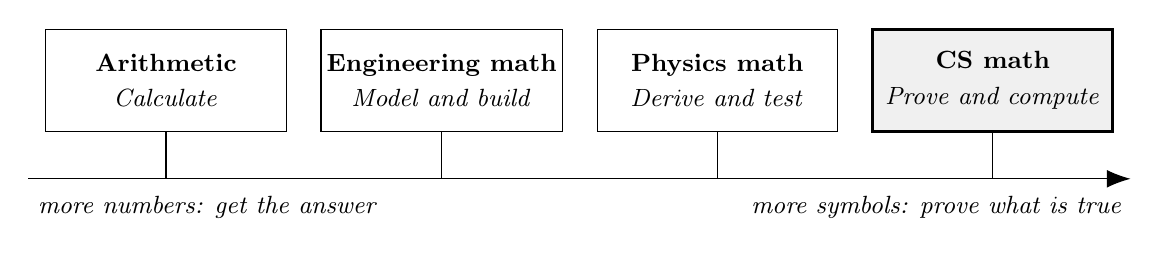
\begin{tikzpicture}[
  box/.style={draw, minimum width=3.05cm, minimum height=1.3cm, inner xsep=2pt, align=center, font=\small},
  x=3.5cm]
  \foreach \i/\name/\verb in {0/Arithmetic/Calculate, 1/Engineering math/Model and build,
                              2/Physics math/Derive and test} {
    \node[box] (b\i) at (\i,0) {\textbf{\name}\\[0.2em]\textit{\verb}};
    \draw (b\i.south) -- (\i,-1.25);
  }
  \node[box, fill=gray!12, line width=1.1pt] (b3) at (3,0) {\textbf{CS math}\\[0.2em]\textit{Prove and compute}};
  \draw (b3.south) -- (3,-1.25);
  \draw[-{Latex[length=3mm]}] (-0.5,-1.25) -- (3.5,-1.25);
  \node[anchor=north west, font=\small\itshape] at (-0.5,-1.35) {more numbers: get the answer};
  \node[anchor=north east, font=\small\itshape] at (3.5,-1.35) {more symbols: prove what is true};
\end{tikzpicture}
\caption*{\itshape Figure 1 -- From numbers to symbols, as placed in these notes}
\end{figure}

% =====================================================================
\section{Reasoning in Chunks}
% =====================================================================

Memorizing and chunking are different things. Recall pulls a stored answer out of memory.
Chunking packs many small pieces into one bigger piece that working memory can hold as a
single unit. Miller put the span of immediate memory at about seven items, plus or minus two,
and described recoding into chunks as a way around that limit. \cite{miller} An observation from these
notes: a lot of everyday CS notation looks like chunking.

\newpage % page break as in original (p6)
\begin{itemize}
  \item \textbf{Hex works like chunking.} Eight loose bits sit near the upper end of that span. Grouped
        into two 4-bit nibbles, they become two symbols: 1010 0011 is just A3. No need to hold
        256 values, only two chunks of sixteen.
  \item \textbf{Powers are chunked multiplication.} $2^{10}$ is ten doublings packed into one symbol, and it
        is about 1000. So $2^{20}$ is about a million and $2^{30}$ about a billion. One way to see it: thinking
        in ``this to the power of that'' is thinking in chunks of repeated multiplication.
  \item \textbf{Abstraction can be read as chunking at scale.} A function hides its steps behind a name,
        a network stack hides each layer's details from the layer above.
\end{itemize}

\gfnote{im notorious for my terrible memory. i forget the binary table, i forget
bron-kerbosch, hell, i even forget the times tables\ldots\ but i can reason the 256 table, to the
power of this and that and so on, kinda. its like chunking, look at hex for example.}

\begin{table}[H]
\centering
\caption*{\itshape Table 3 -- Hex: one symbol per 4-bit chunk}
\footnotesize
\setlength{\tabcolsep}{2.6pt}
\begin{tabular}{@{}l*{16}{c}@{}}
\toprule
\textbf{Hex} & 0 & 1 & 2 & 3 & 4 & 5 & 6 & 7 & 8 & 9 & A & B & C & D & E & F \\
\midrule
\textbf{Binary} & 0000 & 0001 & 0010 & 0011 & 0100 & 0101 & 0110 & 0111 & 1000 & 1001 & 1010 & 1011 & 1100 & 1101 & 1110 & 1111 \\
\bottomrule
\end{tabular}
\end{table}

Sixteen entries make up the whole table, and you never need more, because every byte is just
two of these chunks side by side:

\begin{center}
\texttt{1101 1110 1010 1101 1011 1110 1110 1111 $\rightarrow$ DE AD BE EF}
\end{center}

Thirty-two bits, hard to hold as loose digits, become eight symbols, four bytes, read in one
glance. Same trick in reverse: to turn 0xA3 into binary, look up A (1010) and 3 (0011) and
glue them, 1010 0011. No 256-row table, just one 16-entry table used twice.

And the tables can always be rebuilt from their rule:

\begin{itemize}
  \item \textbf{Powers of 2:} keep doubling. 1, 2, 4, 8, 16, 32, 64, 128, 256.
  \item \textbf{Binary:} each bit position is one of those doubled values. $1011 = 8 + 0 + 2 + 1 = 11$. Eight
        place values, never a 256-row table.
  \item \textbf{Times tables:} break the problem apart. $7 \times 8 = 7 \times 10 - 7 \times 2 = 70 - 14 = 56$. Slower,
        always correct.
\end{itemize}

% =====================================================================
\section{Closing}
% =====================================================================

To sum up what these notes observed: the math behind CS is mostly discrete mathematics and
logic, built up into algorithms and complexity, and topped by the theory of what can be
computed. It is done with computation in mind and is often checked by proof or by code that
runs. Engineering and physics work more with continuous mathematics and check themselves
against how things actually behave. Arithmetic is the ground beneath all of them. The lines
blur constantly: digital engineering runs on logic, and embedded systems uses both, calculus
for the circuits and signals, discrete mathematics for the logic and the code.

\newpage % page break as in original (p7)
\gfnote{i am not a mathematician. i am a guy with a notebook who got curious about
what the machine is actually doing underneath. if a reasoning here is off, good, noticing is how
it gets better, not noticing is worse\ldots.}

\noindent\rule{\textwidth}{0.6pt}

% =====================================================================
% References
% =====================================================================
\begingroup
\renewcommand{\section}[2]{}% suppress default heading
\begin{center}
{\bfseries REFERENCES}
\end{center}
\vspace{-0.8em}
\small
\begin{thebibliography}{15}
\setlength{\itemsep}{0.1em}

\bibitem{rosen} K. H. Rosen, \textit{Discrete Mathematics and Its Applications}, 8th ed. New York: McGraw-Hill, 2019.

\bibitem{rsa} R. L. Rivest, A. Shamir, and L. Adleman, ``A Method for Obtaining Digital Signatures and Public-Key
Cryptosystems,'' \textit{Communications of the ACM}, vol. 21, no. 2, pp. 120--126, 1978.

\bibitem{knuth} D. E. Knuth, \textit{The Art of Computer Programming, Vol. 1: Fundamental Algorithms}. Reading, MA:
Addison-Wesley, 1968.

\bibitem{turing} A. M. Turing, ``On Computable Numbers, with an Application to the Entscheidungsproblem,''
\textit{Proceedings of the London Mathematical Society}, s2-42, pp. 230--265, 1936.

\bibitem{sipser} M. Sipser, \textit{Introduction to the Theory of Computation}. Boston: PWS Publishing, 1997.

\bibitem{peano} G. Peano, \textit{Arithmetices principia, nova methodo exposita}. Turin: Bocca, 1889.

\bibitem{rudin} W. Rudin, \textit{Principles of Mathematical Analysis}. New York: McGraw-Hill, 1953.

\bibitem{aristotle} Aristotle, \textit{Prior Analytics}, c. 350 BC.

\bibitem{euclid} Euclid, \textit{Elements}, c. 300 BC.

\bibitem{mates} B. Mates, \textit{Stoic Logic}. Univ. of California Publications in Philosophy, vol. 26. Berkeley: UC Press,
1953.

\bibitem{boole} G. Boole, \textit{The Mathematical Analysis of Logic}. Cambridge: Macmillan, Barclay, and Macmillan, 1847;
\textit{The Laws of Thought}. London: Walton and Maberly, 1854.

\bibitem{frege} G. Frege, \textit{Begriffsschrift}. Halle: Louis Nebert, 1879.

\bibitem{shannon} C. E. Shannon, ``A Symbolic Analysis of Relay and Switching Circuits,'' \textit{Transactions of the AIEE}, vol.
57, no. 12, pp. 713--723, 1938.

\bibitem{miller} G. A. Miller, ``The Magical Number Seven, Plus or Minus Two,'' \textit{Psychological Review}, vol. 63, no. 2,
pp. 81--97, 1956.

\bibitem{smith} R. Smith, ``Aristotle's Logic,'' in \textit{The Stanford Encyclopedia of Philosophy}, E. N. Zalta, ed. Stanford
University, first published 2000.

\end{thebibliography}
\endgroup

\gfnote{the machine does the counting. my job is knowing why the count is right.}

\begin{flushright}
GreyFox\\
\textit{Jibaro Archives, 2026}
\end{flushright}

\end{document}
